% -*- TeX-engine: default; TeX-PDF-mode: t; -*-
\ifdefined\pdfoutput
  \pdfoutput=1
\fi
\documentclass[12pt,letterpaper]{article}

%% === margins / layout ===
\usepackage{iftex}
\ifPDFTeX
  \pdfminorversion=4
  \PassOptionsToPackage{pdftex}{hyperref}
\fi
\usepackage[margin=1in]{geometry}

%% === basic packages ===
\ifPDFTeX
  \usepackage[T1]{fontenc}
  \usepackage[utf8]{inputenc}
  \usepackage{lmodern}
\else
  \usepackage{fontspec}
  \setmainfont{Times New Roman}
  \setsansfont{Helvetica}
  \setmonofont{Menlo}
  % Render non-Latin scripts in trace tables without manual font switching.
  \ifXeTeX
    \usepackage{ucharclasses}
    \newfontfamily\armenianfont{Mshtakan}
    \setTransitionsFor{Armenian}{\armenianfont}{\normalfont}
  \fi
\fi
\usepackage{microtype}
\usepackage{latexsym}
\usepackage{amssymb,amsmath,bm}
\usepackage{mathtools}
\usepackage{booktabs}
\usepackage{graphicx}
\usepackage{float}
\usepackage{enumitem}
\usepackage{setspace}
\usepackage{placeins}
\newcommand\spacingset[1]{\setstretch{#1}}

%% === tables for trace examples ===
\usepackage{ragged2e}
\usepackage{tabularx}
\usepackage[table]{xcolor}
\usepackage{threeparttable}
\definecolor{RowShade}{gray}{0.96}
\newcolumntype{P}[1]{>{\RaggedRight\arraybackslash}p{#1}}
\newcolumntype{C}[1]{>{\Centering\arraybackslash}p{#1}}
\newcolumntype{Y}{>{\RaggedRight\arraybackslash}X}

%% === hyperlinks ===
\usepackage[bookmarksopen=true, bookmarksnumbered=true,
pdfstartview=FitH, breaklinks=true,
urlbordercolor={0 1 0}, citebordercolor={0 0 1}]{hyperref}

%% === TikZ ===
\usepackage{tikz}
\usetikzlibrary{arrows.meta,calc,positioning,fit,shapes.geometric,shapes.misc,backgrounds}

%% === bibliography ===
\usepackage[natbib=true,minnames=1,maxnames=3,backend=biber,style=authoryear-luh-ipw]{biblatex}
\IfFileExists{mybib.bib}{
  \addbibresource{mybib.bib}
}{
  \addbibresource{asa-paper/Paper/mybib.bib}
}

%% === figure path ===
\graphicspath{{./../Figures/}{asa-paper/Paper/../Figures/}}
\makeatletter
\def\input@path{{./}{asa-paper/Paper/}}
\makeatother

%% === stats macros (generated) ===
\InputIfFileExists{./../Figures/LLM_pol_party_Statistics.tex}{}{
  \newcommand{\LLMOverallAccAllpolparty}{0.751}
\newcommand{\LLMOverallAccHighpolparty}{0.860}
\newcommand{\LLMMeanLowConfpolparty}{0.250}
\newcommand{\LLMMedianLowConfpolparty}{0.250}
\newcommand{\LLMMeanAccByCountryHighpolparty}{0.879}
\newcommand{\LLMMeanBaselineByCountrypolparty}{0.536}
\newcommand{\LLMMeanDeltaByCountrypolparty}{0.343}
\newcommand{\LLMMinDeltaByCountrypolparty}{-0.602}
\newcommand{\LLMMaxDeltaByCountrypolparty}{0.761}
\newcommand{\LLMMinDeltaCountrypolparty}{Gambia}
\newcommand{\LLMMaxDeltaCountrypolparty}{Finland}
\newcommand{\LLMMeanAccSmallGroupspolparty}{0.692}
\newcommand{\LLMMeanAccLargeGroupspolparty}{0.820}
\newcommand{\LLMNumCountriespolparty}{114}
\newcommand{\LLMNumInstancespolparty}{34,618}
\newcommand{\LLMNumClassespolparty}{1,209}
\newcommand{\LLMNumPredictionsGainedpolparty}{12,898}
\newcommand{\LLMNumPredictionsGainedPercentpolparty}{20.8}
\newcommand{\LLMRelaxedChangedPctpolparty}{2.5}

}

\title{An Auditable Search Agent Methodology at Scale for Political Elite Research}
\author{Connor T. Jerzak \& Team (Final author list TBD)}
\date{}

\begin{document}
\maketitle
\spacingset{1}

\begin{abstract}
\noindent Large-\(N\) political-elite datasets increasingly rely on digital traces, but scaling elite attribute coding with search-enabled LLMs can undermine auditability, cross-national comparability, and temporal validity.
We propose an \emph{auditable search agent} (ASA) protocol that treats web retrieval as a governed measurement instrument.
For each \(\langle\)person, country, year\(\rangle\) record, ASA runs a short search session, constrains outputs to expert closed codebooks, enforces an ``as-of'' evidence rule, abstains under weak or conflicting support, and archives complete provenance (queries, snippets, URLs, timestamps).
In a party-affiliation labeling task spanning
\LLMNumCountriespolparty{} countries (\(N=\)
\LLMNumInstancespolparty{} leader--records; \LLMNumClassespolparty{}
labels), ASA attains \LLMOverallAccHighpolparty{} accuracy on
high-evidence cases while increasing usable coverage by
\LLMNumPredictionsGainedPercentpolparty{}\% through conservative
augmentation. The agent design is general and, we hope, could have applicability in other data collection domains where web retrieval is informative. 
\end{abstract}
\vspace{0.4em}
\noindent\textbf{Keywords:} political elites; measurement; tool-using
retrieval; replication; temporal leakage.

\vspace{0.5cm}

\noindent Note! Extremely preliminary. 

\spacingset{1}

\section{Introduction}

Large-\(N\) political-elite datasets underpin research on representation, accountability, and governance, but assembling them requires repeated, error-prone measurement of categorical attributes (e.g., party affiliation) across countries and time.
As digital traces proliferate, it is tempting to scale attribute coding by asking search-enabled large language models (LLMs) for answers.
Yet, interactive question answering is not a measurement protocol: without explicit governance, such workflows tend to be difficult to audit, hard to replicate, and vulnerable to temporally invalid evidence.

The stakes are substantive, not only technical. Party affiliation and related elite attributes are widely used to define key covariates (e.g., partisan control, coalition membership, and ideological composition) and to subset samples (e.g., focusing on elected officials with identifiable party ties). When labels are missing or miscoded, downstream analyses can suffer selection bias and reduced comparability across countries and years; when labels are coded using post-period biographies or retrospective summaries, they risk post-\(t\) contamination of baseline covariates.

In political methodology terms, the problem is therefore \emph{measurement design}: how do we scale coding of elite attributes while preserving (i) auditability (a third party can verify why a label was produced), (ii) cross-national comparability (labels remain in a stable, closed set of classes), and (iii) temporal validity (evidence respects an ``as-of'' target).
ASA is framed as a measurement protocol rather than as an accuracy-maximizing question-answering system.

We argue that search-augmented LLM agents can be most useful for dataset construction when embedded in an explicitly governed measurement protocol where source temporality can be controlled and provenance can be carefully studied.
We introduce the \emph{Auditable Search Agent} (ASA), implemented in the \texttt{asa} software stack, which formalizes retrieval as measurement: for each record \(\langle\)person, country, year\(\rangle\) and an expert-supplied closed codebook, the agent runs a short, budgeted search session; prioritizes evidence over parametric recall; emits a structured output with citations; abstains under weak or conflicting evidence; and archives a complete trace (queries, snippets, URLs, timestamps) for later audit and re-analysis.

We aim to make three key contributions. First, we identify three hazards that threaten LLM-only inference in research workflows: (i) non-verifiability, (ii) non-comparability, and (iii) temporal leakage (a close analogue to post-treatment conditioning in causal inference). Second, to mitigate these hazards, we introduce a concrete protocol emphasizing closed-world decisions, evidence-first outputs, temporal governance, and conservative abstention. Third, we validate this methodology using party-affiliation labeling—a verifiable elite attribute governed by an expert, closed codebook.

Previewing results -- in the party-affiliation task spanning \LLMNumCountriespolparty{} countries (\(N=\) \LLMNumInstancespolparty{} matched leader--records; \LLMNumClassespolparty{} party labels), ASA achieves high-confidence accuracy \LLMOverallAccHighpolparty{} while expanding usable coverage by \LLMNumPredictionsGainedPercentpolparty{}\% (\LLMNumPredictionsGainedpolparty{} previously missing labels) and withholding \LLMMeanLowConfpolparty{} of cases on average via an abstention gate.
Relative to a simple country-majority baseline (\LLMMeanBaselineByCountrypolparty{}), the mean uplift in high-confidence accuracy is \LLMMeanDeltaByCountrypolparty{}.

Next, Section~\ref{sec:hazards} motivates the design by formalizing three measurement hazards.
Section~\ref{sec:related} situates the contribution in political methodology, reproducible research, and recent retrieval-agent architectures.
Sections~\ref{sec:method}--\ref{sec:validation} describe the ASA protocol and validate it on party affiliation.
We conclude with guidance on transparency, limitations, and ethical considerations for web-based measurement.
Our replication target is recomputation from a frozen trace store and versioned task specification; we do not claim that reruns on the live web will match.

\section{Measurement hazards in search-enabled coding\label{sec:hazards}}

Digital sources make it feasible to code political-elite attributes at scale, but research-grade datasets impose requirements that differ from interactive question answering.
In practice, a default workflow---``ask a LLM model for the answer''---tends to fail on three dimensions central to quantitative political science.

\paragraph{Auditability and replication.}
Elite attribute labels are \emph{measurements}. When the underlying retrieval context is not archived (queries, results, snippets, URLs, timestamps), a label is difficult to verify and cannot be re-audited when coders disagree or sources change.
This is especially problematic for downstream users who need to understand measurement error and may wish to apply alternative inclusion rules (e.g., discarding any label lacking a primary source).

\paragraph{Cross-national comparability.}
Many elite variables are \emph{categorical} and country-specific (e.g., party labels). ``Open-world'' generation invites label drift (synonyms, translations, rebrandings), undermining comparability across countries and years.
Closed codebooks supplied by domain experts are a natural remedy, but generic chat systems do not typically enforce them.

\paragraph{Temporal leakage and post-treatment bias.}
Political elites switch parties, offices, and coalitions. If coding
for year \(t\) uses sources written after \(t\) (e.g., biographies
updated in 2025), the measurement can incorporate information that is
itself caused by post-\(t\) outcomes.

This is a close analogue of conditioning on post-treatment variables in causal inference \citep{montgomery2018conditioning}: a label intended to reflect the pre-period state may be contaminated by later events, inducing bias in estimated relationships.
Temporal governance therefore belongs \emph{inside} the measurement protocol, not in ad hoc post-hoc cleaning.

\subsection{Formalizing temporal leakage\label{sec:temporal-formal}}

The third concern regarding post-treatment information is particularly acute in LLM-only coding, as the LLM weights have been trained extensively with post treatment information. We here briefly formalize the structural relationship between the target attribute, downstream outcomes, and the evolving data-generating process of web evidence. By explicitly mapping the timeline of information retrieval, we can establish a compliance rule that isolates the pre-period state from future events, ensuring the agent's measurements remain valid for downstream inference.

Let \(X_{it}\) denote the target attribute for unit \(i\) at time \(t\) (e.g., party affiliation in observation year \(t\)).
Researchers often use \(X_{it}\) as a covariate when estimating relationships with outcomes realized after \(t\), \(Y_{i,t'>t}\).
Web-based coding observes a set of sources \(S_{it}\) whose content and availability depend on time: some sources are available at or before \(t\) (\(S^{\le t}_{it}\)), while others are published or updated after \(t\) (\(S^{>t}_{it}\)).
When a measurement procedure for \(X_{it}\) draws on \(S^{>t}_{it}\), it can implicitly incorporate information downstream of \(Y_{i,t'>t}\) (e.g., retrospective biographies updated after a party switch), creating look-ahead leakage and a close analogue of post-treatment conditioning.\footnote{See \citet{paleka2025pitfalls} for a broader discussion of temporal validity pitfalls when ``as-of'' constraints are not enforced in evaluation settings.}

\begin{figure}[htb]
  \centering
  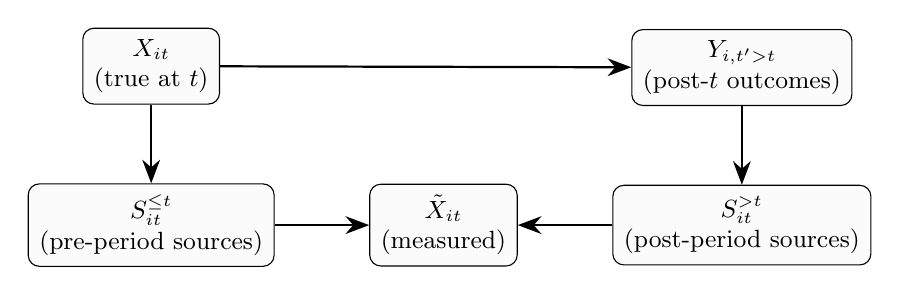
\begin{tikzpicture}[
    font=\small,
    node distance=10mm and 12mm, % Adjusted horizontal distance slightly for a 3-column layout
    v/.style={draw, rounded corners, fill=gray!3, inner sep=4pt, align=center},
    arr/.style={-{Stealth[length=3mm]}, thick},
  ]
    % Left side
    \node[v] (x) {\(X_{it}\)\\(true at \(t\))};
    \node[v, below=of x] (spre) {\(S^{\le t}_{it}\)\\(pre-period sources)};

    % Middle (Collider)
    \node[v, right=of spre] (xhat) {\(\tilde X_{it}\)\\(measured)};

    % Right side
    \node[v, right=of xhat] (spost) {\(S^{>t}_{it}\)\\(post-period sources)};
    \node[v, above=of spost] (y) {\(Y_{i,t'>t}\)\\(post-\(t\) outcomes)};

    % Arrows
    \draw[arr] (x) -- (y);
    \draw[arr] (x) -- (spre);
    \draw[arr] (y) -- (spost);
    \draw[arr] (spre) -- (xhat);
    \draw[arr] (spost) -- (xhat);
  \end{tikzpicture}
  \caption{Temporal leakage as post-period conditioning. If measurement \(\tilde X_{it}\) uses post-period sources \(S^{>t}_{it}\) that are themselves influenced by outcomes after \(t\), then \(\tilde X_{it}\) can become a function of \(Y_{i,t'>t}\), contaminating a baseline covariate.}
  \label{fig:temporal-dag-alt}
\end{figure}

\paragraph{A compliance definition.}
For each record \(i\), the task specification includes a temporal cut \(\tau_i\) (an ``as-of'' date).
Each retrieved source \(s \in S_{it}\) is assigned a best-effort publication (or last-update) date \(d(s)\) when recoverable.
Define the admissible evidence set \(S^{\mathrm{adm}}_{it}(\tau_i)=\{s \in S_{it}: d(s)\ \text{exists and}\ d(s)\le \tau_i\}\).
ASA treats a label as \emph{temporally compliant} only if (i) its cited supporting sources are drawn from \(S^{\mathrm{adm}}_{it}(\tau_i)\), and (ii) at least one cited supporting source has a recoverable \(d(s)\).
When no supporting source has a recoverable date, ASA downgrades evidence strength and abstains rather than silently relying on potentially post-period material.

\paragraph{Design implications.}
These hazards motivate treating retrieval as a governed measurement instrument: decisions must be constrained (closed codebooks), evidence must be preserved (citations and traces), time must be part of the protocol (``as-of'' rules), and weak evidence should trigger abstention rather than guessing.
Table~\ref{tab:hazard-mitigation} summarizes how ASA operationalizes these requirements.

\begin{table}[htb]
\centering
\caption{Common hazards in search-enabled coding and ASA design responses.}
\label{tab:hazard-mitigation}
\small
\begin{tabularx}{\linewidth}{@{}>{\RaggedRight\arraybackslash}p{0.30\linewidth}X@{}}
\toprule
\textbf{Hazard} & \textbf{ASA response} \\
\midrule
Non-verifiability (answers without durable evidence trails) &
                                                              Evidence-first outputs with explicit citations; full trace capture (queries, snippets, URLs, timestamps) for audit and re-analysis. \\
 & & \\ 
Non-comparability (label drift across countries/time) &
                                                        Closed-world decisions constrained to expert codebooks, plus conservative post-processing that normalizes benign surface variation without introducing new classes. \\
   & & \\ 
Temporal leakage (post-period information used for pre-period labels) &
Explicit ``as-of'' rules with date verification where feasible; warnings and abstention rather than silently relying on potentially post-period sources. \\
\bottomrule
\end{tabularx}
\end{table}

\subsection{Auditability and comparability as formal properties\label{sec:formal-audit-compare}}

Temporal leakage is only one way search-enabled coding can fail as measurement.
To make retrieval an admissible instrument for political data construction, we also require
(1) \emph{auditability} (a third party can reconstruct why a label was emitted) and
(2) \emph{comparability} (outputs remain in a stable, closed set of classes across country-years).

\paragraph{The trace as the measurement object.}
Let \(\Omega_t\) denote the (unobserved) state of the web at time \(t\).
A tool-using coding episode for record \(i\) produces a \emph{trace}
\[
  T_i = \big( (a_{i1}, o_{i1}, \kappa_{i1}), \ldots, (a_{iK}, o_{iK}, \kappa_{iK}) \big),
\]
where each step records the agent action \(a_{ik}\) (e.g., a query or page fetch),
the observed tool output \(o_{ik}\) (e.g., ranked results and extracted snippets), and a timestamp \(\kappa_{ik}\).
The reported label is a function of the trace and the task specification:
\[
  \hat{X}_{it} = M(T_i;\,\mathcal{C}_i,\tau_i,E,\theta),
\]
where \(\mathcal{C}_i\) is the closed codebook, \(\tau_i\) is the temporal cut,
\(E\) is an evidence sufficiency rule, and \(\theta\) denotes implementation parameters
(e.g., mapping thresholds and source-tier rules).

\paragraph{Auditability.}
We say a coding procedure is \emph{auditably reproducible} for a reported result if,
given a \emph{frozen} trace store \(\mathcal{T}=\{T_i\}_{i=1}^N\) and a versioned task specification
\((\mathcal{C}_i,\tau_i,E,\theta)\), an independent auditor can deterministically recompute every
reported label and every aggregate statistic in the paper by replaying \(M(\cdot)\) on \(\mathcal{T}\).
This is the relevant reproducibility target for web-based measurement: rerunning retrieval on the live web
is not expected to match, but recomputation from an archived trace store is.\footnote{This distinction mirrors a broader point in agentic systems: raw action logs are often insufficient for claim-level auditability without structured, claim--evidence encodings \citep{rasheed2026fluent}.}

\paragraph{Comparability via closed-world mapping.}
Cross-national comparability requires that categorical labels be stable and enumerable.
ASA enforces a closed-world constraint by requiring \(\hat{X}_{it}\in\mathcal{C}_i\) or abstention.
Let \(g(\cdot)\) map extracted surface strings from evidence into codebook entries.
Closed-world comparability requires \(g\) to be \emph{non-expansive}: it may normalize benign surface variation
(punctuation, spacing, acronyms) but must never introduce a class outside \(\mathcal{C}_i\).
When \(g\) is undefined, or evidence supports multiple codebook entries, ASA abstains rather than generating a novel label.
This operationalizes a basic measurement-validity principle: prefer explicit, auditable missingness to uncontrolled label drift that silently changes the meaning of a variable across units and time \citep{adcock2001measurement,munck2002conceptualizing,lazer2014parable}.

\section{Related work\label{sec:related}}

Our contribution sits at the intersection of political methodology and recent advances in retrieval-augmented language models.
Large cross-national datasets often rely on expert coding and bespoke compilation efforts; a central challenge is preserving comparability and documenting measurement decisions at scale.
ASA complements such efforts by treating web retrieval as a first-class part of the measurement protocol and by archiving evidence trails that allow downstream users to audit labels and re-apply inclusion rules.
The validation task we study is motivated by the same large-\(N\) political-elite measurement agenda that underlies recent work on global leadership and expert-coded cross-national datasets \citep{gerring2019rules,pemstein2020v}.

The political-science measurement literature emphasizes that validity hinges on transparent linkages between concepts, operational rules, and observed indicators, and that measurement choices must be documented in a way that supports reinterpretation and audit.
ASA's closed codebooks, explicit abstention boundary, and trace-based audit target these concerns \citep{adcock2001measurement,munck2002conceptualizing}.
More broadly, digital trace data can be alluring but unstable; classic warnings about shifting data-generating processes in ``big data'' settings apply directly to web-based measurement \citep{lazer2014parable}.

ASA is also aligned with transparency and replication norms in political science, where the goal is not merely to share code but to make measurement decisions inspectable and contestable.
Calls for data access and research transparency (DA-RT), ``active citation,'' and practical guidance on code-and-data release motivate our emphasis on archivable evidence and replayable rules \citep{dart2015joint,moravcsik2014transparency,gentzkow2014code}.

Finally, ASA's abstention gate connects to a long literature on the error--reject tradeoff in recognition systems and to modern selective prediction work that treats abstention as a principled way to control risk \citep{chow1970reject,geifman2017selective}.

ASA is also aligned with calls for reproducible computational research: replication requires not only code, but durable documentation of the information environment that produced a label \citep{peng2011reproducible,stodden2013toward}.
In web-based measurement, the information environment is inherently dynamic; capturing queries, snippets, URLs, and timestamps makes it possible to re-audit outputs when sources change.
Our emphasis on temporal governance connects directly to concerns about look-ahead and leakage when post-period information is used to measure pre-period covariates \citep{kaufman2012leakage,montgomery2018conditioning}.

On the NLP side, retrieval-augmented generation and tool-using agents provide building blocks for ASA's implementation \citep{lewis2020retrieval,yao2022react}.
However, the core contribution here is not a new prompting trick or a larger model; it is a measurement-oriented design that prioritizes comparability, auditability, and temporal validity over unconstrained answer generation.

\section{Methodology: an auditable search agent\label{sec:method}}

We present a protocol---implemented as the \texttt{asa} software stack---that makes agent-based retrieval \emph{verifiable by construction}.
The methodology separates (i) a task-level specification that defines what constitutes admissible evidence and outputs, from (ii) an implementation that executes the specification and persists traces.

\subsection{Protocol commitments}

The protocol has four core commitments:
\begin{enumerate}[leftmargin=*, itemsep=2pt]
\item \textbf{Closed-world decisions.} All predictions must lie in an expert-supplied codebook (e.g., the parties observed in a country-year panel).
\item \textbf{Evidence-first outputs.} Each label is paired with a terse rationale anchored to explicit source citations.
\item \textbf{Provenance preservation.} The system archives the full interaction trace: queries, tool responses, extracted snippets, URLs, and timestamps.
\item \textbf{Conservative abstention.} Under weak or conflicting evidence, the agent abstains (or routes to humans) rather than guessing.
\end{enumerate}

\subsection{Abstention as selective measurement\label{sec:selective-measurement}}

ASA's abstention rule is not merely an implementation detail; it defines the statistical object that is being produced.
Let \(Y_{it}\) denote the expert-coded party label (when available).
ASA returns a \emph{selective} prediction \(\hat{Y}_{it}\in \mathcal{C}_i \cup \{\bot\}\), where \(\bot\) denotes abstention.
Two quantities therefore matter jointly:
\[
  \text{Coverage} \;\gamma \equiv \Pr(\hat{Y}_{it}\neq \bot),
  \qquad
  \text{Conditional error} \; R \equiv \Pr(\hat{Y}_{it}\neq Y_{it}\mid \hat{Y}_{it}\neq \bot).
\]
Tightening evidence requirements mechanically reduces \(R\) while lowering \(\gamma\), an instance of the classic error--reject tradeoff \citep{chow1970reject} and closely related to modern selective classification \citep{geifman2017selective}.
In elite measurement settings, abstention is attractive because withheld cases can be routed to human coders or left missing under transparent, replayable rules---a preferable failure mode to un-auditable guesswork.

\subsection{Task formalization}

For each target record \(i\), the inputs are: a person name, a target country, an observation year \(t_i\), and a closed codebook \(\mathcal{C}_i\) supplied by expert coders.
The agent must return either (a) a label \(c \in \mathcal{C}_i\) with citations, or (b) an abstention.

\begin{figure}[htb]
  \centering
  \fbox{\begin{minipage}{0.95\linewidth}
  \small
  \begin{spacing}{1}
  \textbf{Protocol 1 (ASA): governed retrieval as measurement.}
  \begin{enumerate}[leftmargin=*, itemsep=2pt]
    \item \textbf{Inputs.} Record \(r_i=\langle\)person, country, year\(t_i\rangle\); expert codebook \(\mathcal{C}_i\); temporal cut \(\tau_i\) (``as-of''); retrieval budget \(B\); and an evidence sufficiency rule \(E\) (task-specified).
    \item \textbf{Retrieve (trace everything).} Issue up to \(B\) read-only retrieval actions (e.g., Wikipedia + web search). Persist each query, ranked results, extracted snippets, URLs, and timestamps.
    \item \textbf{Date and filter sources.} For each candidate source \(s\), recover a publication/last-update date \(d(s)\) when feasible. Mark sources with \(d(s)>\tau_i\) as post-period and inadmissible for a high-evidence decision; mark sources without recoverable \(d(s)\) as undated.
    \item \textbf{Extract candidate labels.} From admissible snippets, extract party-name strings and map to \(\mathcal{C}_i\) via strict match, then conservative fuzzy normalization for benign surface variation.
    \item \textbf{Decide or abstain.} If mapped evidence meets \(E\) using admissible sources and does not conflict, output \(c\in\mathcal{C}_i\) with a one-sentence, citation-backed justification and an evidence-strength tier. If evidence is weak, conflicting, or only undated, abstain.
    \item \textbf{Persist artifacts.} Write the structured output (including abstentions) and a pointer to the full trace store entry so results can be re-audited and aggregate statistics recomputed from the frozen trace store.
  \end{enumerate}
  \end{spacing}
  \end{minipage}}
  \caption{A submission-ready ASA protocol statement. The task configuration specifies \(\mathcal{C}_i\), \(\tau_i\), \(B\), and \(E\); the shared execution layer enforces trace capture, temporal admissibility, and abstention.}
  \label{fig:asa-protocol}
\end{figure}

\subsection{Evidence sufficiency and confidence tiers\label{sec:evidence-rule}}

The protocol parameter \(E\) encodes what counts as \emph{sufficient evidence} for emitting a high-confidence label.
In party-affiliation coding, we implement \(E\) as a tiered evidence rule that privileges primary, contemporaneous sources and requires independence across sources.

\paragraph{Source tiers.}
Each retrieved source \(s\) is assigned a coarse reliability tier---primary, secondary, or tertiary---using domain lists and page cues.
We treat \emph{primary/official} sources (e.g., government, parliament, election commission, party roster pages) as the strongest evidence; \emph{secondary} sources include major news outlets and established reference works; \emph{tertiary} sources (e.g., scraped bios and low-editability directories) may be used for navigation but are not, by themselves, sufficient for high-evidence decisions.

\paragraph{Independence.}
To reduce correlated error, we treat two sources as independent if they come from different base domains and are not obvious mirrors or syndicated copies.
This criterion is deliberately coarse but easy to audit in stored traces.

\paragraph{Tiered sufficiency rule.}
Let \(S^{\mathrm{adm}}_{it}(\tau_i)\) be the admissible (dated, pre-\(\tau_i\)) evidence set defined in Section~\ref{sec:temporal-formal}.
ASA assigns each record to one of three evidence tiers:
\begin{enumerate}[leftmargin=*, itemsep=2pt]
\item \textbf{Tier A (high evidence):} At least two independent admissible sources map non-expansively to the same codebook label, including at least one primary/official source with a recoverable date.
\item \textbf{Tier B (moderate evidence):} Either (i) one admissible primary/official source maps cleanly to a label, or (ii) two independent secondary sources agree, but primary evidence is unavailable.
\item \textbf{Tier C (weak/undated/conflicting):} Evidence is undated, post-period, maps to multiple labels, or relies only on tertiary sources.
\end{enumerate}
In our default configuration we emit a high-confidence label only under Tier A; Tier B is available for human review or sensitivity checks; Tier C cases are abstentions.
This makes the abstention boundary explicit and replayable: downstream users can tighten or relax \(E\) and recompute headline statistics from the same frozen trace store.

\begin{table}[htb]
\centering
\caption{Evidence tiers used by the sufficiency rule \(E\) in party-affiliation coding.}
\label{tab:evidence-tiers}
\small
\begin{tabularx}{\linewidth}{@{}lP{2.9cm}X@{}}
\toprule
\textbf{Tier} & \textbf{Minimum sources} & \textbf{Operational rule (summary)} \\
\midrule
A (high evidence) & \(\ge 2\) independent & Dated, admissible sources agree on the mapped codebook label; includes \(\ge 1\) primary/official source with recoverable date; no unresolved conflict. Emit a high-confidence label. \\
B (moderate evidence) & \(1\) primary or \(2\) secondary & Agreement under admissible dating, but primary evidence is limited or unavailable. Route to human review or treat as medium confidence in sensitivity checks. \\
C (weak / conflicting) & -- & Evidence is undated or post-period, relies on tertiary sources, or supports multiple labels with comparable strength. Abstain. \\
\bottomrule
\end{tabularx}
\end{table}

\subsection{Conflict policy: resolve or abstain\label{sec:conflict-policy}}

Conflicts arise when two different codebook labels are each supported by at least one independent admissible source.
Because post-hoc tie-breaking can silently encode researcher discretion, ASA defaults to abstention under conflict unless one label strictly dominates by evidence tier (e.g., Tier A support versus Tier B/C) and source tier (primary versus secondary/tertiary).
All conflict flags and supporting citations are persisted so disagreements are auditable and can be routed to human coders.

\subsection{Entity disambiguation\label{sec:disambiguation}}

Elite names are not unique: homonyms, transliterations, and office changes can induce systematic misattribution if not governed explicitly.
ASA therefore requires that at least one cited evidence span contain a corroborating identifier beyond the name (e.g., office/chamber, country, year/tenure, or constituency).
When disambiguation remains unresolved, ASA abstains rather than guessing.

\subsection{Implementation: ASA software stack}

Operationally, the agent runs a short search session with read-only retrieval tools (e.g., Wikipedia and general web search), compiles candidate evidence, and emits a structured JSON result (label, one-sentence justification with citations, and a confidence category).
This design follows retrieval-augmented, tool-using agent patterns in the recent NLP literature \citep{yao2022react,lewis2020retrieval}.
The implementation is designed to be \emph{task-configurable}: domain experts supply the closed codebook and task schema, while the shared execution layer enforces the protocol commitments (trace capture, abstention, and evidence-first outputs).

A conservative post-processor then normalizes the label against the codebook: exact-match acceptance first, followed by a guarded fuzzy match for benign surface variation (punctuation, plurals, acronyms) using high similarity thresholds.
This reduces typographic drift without introducing new classes; in the party-affiliation case study, the relaxed mapper changes \LLMRelaxedChangedPctpolparty{}\% of accepted labels.

\begin{figure}[htb]
  \centering
  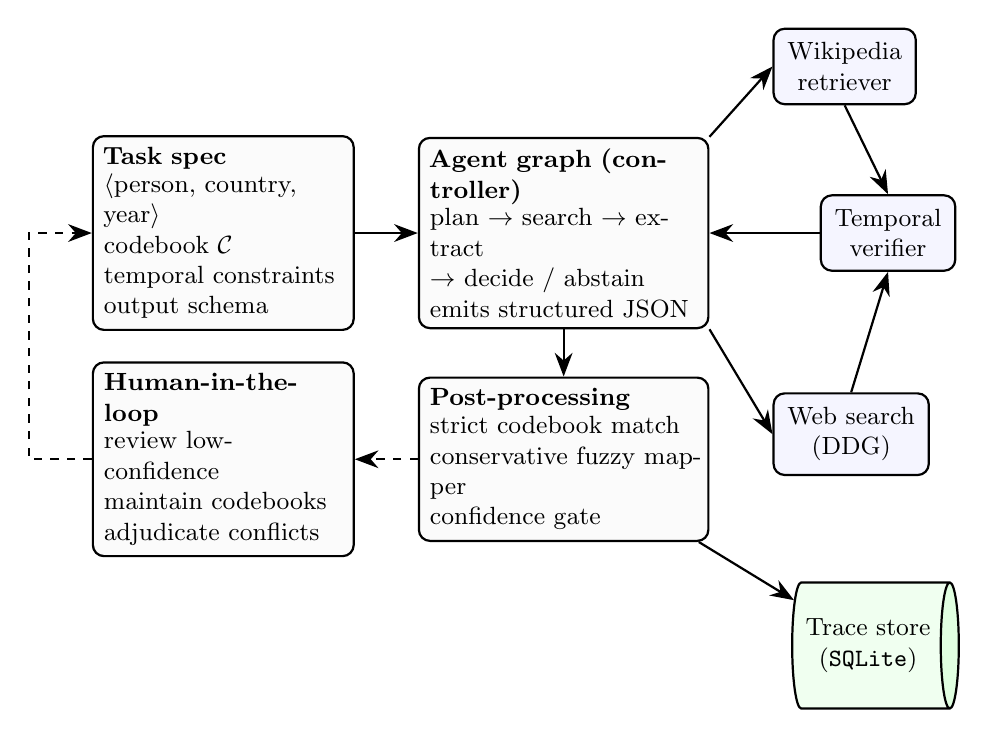
\begin{tikzpicture}[
    font=\small,
    node distance=6mm and 8mm,
    comp/.style={rounded corners, draw=black, thick, fill=gray!3, inner sep=4pt, align=left},
    tool/.style={rounded corners, draw=black, thick, fill=blue!4, inner sep=5pt, align=center},
    store/.style={cylinder, cylinder uses custom fill, cylinder body fill=green!6, cylinder end fill=green!12, draw=black, thick, aspect=0.25, minimum height=18mm, minimum width=16mm, align=center},
    arr/.style={-{Stealth[length=3mm]}, thick},
    loop/.style={-{Stealth[length=3mm]}, thick, dashed},
  ]
    \node[comp, text width=0.25\linewidth] (spec) {
      \textbf{Task spec}\\[-1pt]
      \(\langle\)person, country, year\(\rangle\)\\
      codebook \(\mathcal{C}\)\\
      temporal constraints\\
      output schema
    };

    \node[comp, right=of spec, text width=0.28\linewidth] (graph) {
      \textbf{Agent graph (controller)}\\[-1pt]
      plan \(\rightarrow\) search \(\rightarrow\) extract\\
      \(\rightarrow\) decide / abstain\\
      emits structured JSON
    };

    \node[tool, above right=4mm and 8mm of graph] (wiki) {Wikipedia\\retriever};
    \node[tool, below right=8mm and 8mm of graph] (web) {Web search\\(DDG)};
    \node[tool, right=14mm of graph] (time) {Temporal\\verifier};

    \node[comp, below=of graph, text width=0.28\linewidth] (post) {
      \textbf{Post-processing}\\[-1pt]
      strict codebook match\\
      conservative fuzzy mapper\\
      confidence gate
    };

    \node[store, below right=5mm and 12mm of post] (db) {Trace store\\(\texttt{SQLite})};

    \node[comp, left=of post, text width=0.25\linewidth] (human) {
      \textbf{Human-in-the-loop}\\[-1pt]
      review low-confidence\\
      maintain codebooks\\
      adjudicate conflicts
    };

    \draw[arr] (spec) -- (graph);
    \draw[arr] (graph) -- (post);
    \draw[arr] (post) -- (db);

    \draw[arr] (graph.north east) -- (wiki.west);
    \draw[arr] (graph.south east) -- (web.west);
    \draw[arr] (wiki.south) -- (time.north);
    \draw[arr] (web.north) -- (time.south);
    \draw[arr] (time.west) -- ([xshift=0mm]graph.east);

    \draw[loop] (post.west) -- (human.east);
    % Route this feedback loop outside the "Task spec" box (avoid striking through text).
    \draw[loop] (human.west) -| ([xshift=-8mm]spec.west) -- (spec.west);
  \end{tikzpicture}%
  \caption{Design visualization: a governed agent graph with temporal verification, conservative normalization, abstention, and an auditable trace store.}
  \label{fig:asa-design}
\end{figure}

\subsection{Temporal governance to prevent leakage}

The agent treats time as part of the measurement protocol. Each run is parameterized by an ``as-of'' rule: sources should be published before a cut date (e.g., \(t_i+1\) year) or within a target window around \(t_i\).
When feasible, the system extracts publication dates from retrieved pages and enforces the constraint strictly; otherwise it falls back to best-effort warnings and abstention rather than silently using potentially post-period material.
This guards against a common dataset-construction failure mode: coding pre-period attributes with post-period knowledge.

\paragraph{Operational date recovery \(d(s)\).}
For each retrieved page, ASA attempts to recover a publication or last-update date using an ordered set of heuristics:
(i) structured metadata (e.g., schema.org JSON-LD fields such as \texttt{datePublished}/\texttt{dateModified}),
(ii) HTML meta tags (e.g., OpenGraph/RSS cues),
(iii) visible byline dates in page text, and
(iv) weak URL date patterns as a last resort.
If no reliable date is found, the source is treated as undated and cannot be the sole support for a Tier~A decision (Section~\ref{sec:evidence-rule}).

Temporal controls are crucial because many online sources are retrospective and continuously updated: Wikipedia leads, later biographies, and obituaries often summarize whole careers, including events after \(t_i\). If such post-\(t_i\) material is used to code a pre-period attribute, the measurement can incorporate information that is itself downstream of later outcomes (e.g., a party switch or coalition realignment that occurs after \(t_i\)), creating look-ahead/data leakage and a close analogue of post-treatment conditioning. This can both inflate apparent coding accuracy (by using information unavailable at the time) and bias downstream relationships by contaminating ``baseline'' covariates with post-period events \citep{montgomery2018conditioning,kaufman2012leakage}.

\subsection{Provenance preservation and storage}

All tool interactions and intermediate artifacts are persisted (including URLs and timestamps) to enable:
(i) verification of any individual label by following its citations, (ii) replication of aggregate statistics given the same trace store, and (iii) retrospective audits when codebooks change or new sources appear.
The storage design also supports alternative downstream rules (e.g., only keep labels supported by government sources).

\subsection{Trace schema and audit procedure\label{sec:trace-schema}}

A key claim of ASA is that it produces measurements that are \emph{auditable by construction}.
To make this concrete, the trace store persists two linked objects per record \(i\):

\paragraph{(i) A structured decision record.}
This is the minimal unit needed to reproduce the paper's tables:
\[
  D_i = \{\text{record id},\; \hat{Y}_{it},\; \text{tier},\; \mathcal{C}_i,\; \tau_i,\;
  \text{supporting citations},\; \text{conflict flags},\; \text{software version}\}.
\]
The ``supporting citations'' field points to specific snippet spans within retrieved pages (not only URLs), so an auditor can verify that the cited text supports the mapped codebook label.

\paragraph{(ii) A full interaction trace.}
For each tool call \(k\), we store: query string or URL, ranked results, bounded snippet text, timestamp, domain, recovered publication/update date (if any), and extraction metadata.
Storing bounded snippets rather than full pages reduces privacy and copyright exposure while preserving enough context for audit.
Appendix~\ref{sec:appendix-trace} summarizes the minimum field set.

\paragraph{Audit checklist (replayable).}
Given \((D_i, T_i)\), an auditor can verify a high-confidence label by checking:
(1) all cited sources are admissible under the temporal cut (\(d(s)\le\tau_i\)),
(2) cited spans contain an explicit party mention that maps non-expansively into \(\mathcal{C}_i\),
(3) the required number of independent sources is met for the claimed tier (Section~\ref{sec:evidence-rule}),
and (4) there is no unresolved conflict with similarly supported alternatives (Section~\ref{sec:conflict-policy}).
This moves verification from ``trust the model'' to ``inspect the stored evidence.''

\section{Data and gold standard\label{sec:data}}

We validate ASA on party affiliation, a verifiable elite attribute that is frequently missing in large political-elite panels yet can often be corroborated from public records (party rosters, parliamentary biographies), reputable encyclopedic sources, and contemporaneous news coverage.
The unit of analysis is a leader--record indexed by \(\langle\)person, country, year\(\rangle\).

\subsection{Leader records, temporal scope, and unit construction\label{sec:leader-records}}

We begin from a cross-national panel of political elites assembled as part of the Global Leadership Project research program \citep{gerring2019rules,gerring2024composition}.
From this source we construct leader--records indexed by \(\langle\)person, country, year \(t\rangle\).
The observation year \(t\) defines the temporal target for party affiliation, and each ASA run is parameterized by a record-specific temporal cut \(\tau_i\) (Section~\ref{sec:temporal-formal}).

Because names vary across languages and sources, we retain both the original name string and a normalized form (case-folding, diacritic handling) in the trace store.
This supports downstream audits of homonyms and transliterations (Section~\ref{sec:disambiguation}).

\subsection{Expert labels and codebook construction\label{sec:codebooks}}

For each country-year, domain experts provide a \emph{closed codebook} \(\mathcal{C}_i\) of admissible party labels.
The codebook enforces cross-national comparability by preventing open-ended label generation, while allowing country-specific party systems to be represented without forcing artificial cross-country harmonization.
Operationally, codebooks are versioned and frozen for an ASA run; when party naming conventions evolve (coalitions, mergers, rebrands), codebooks can be updated and prior labels can be re-audited using archived traces.
To reduce conservative normalization error, codebooks may include documented aliases that map non-expansively into canonical labels (Section~\ref{sec:formal-audit-compare}).

Expert party labels used for evaluation come from the underlying expert-coding workflow.
We treat these labels as the gold standard for validation, while emphasizing that ASA's trace store preserves enough evidence to support audits and disagreement adjudication, consistent with measurement best practices \citep{adcock2001measurement,munck2002conceptualizing}.

\subsection{Record linkage and match quality\label{sec:record-linkage}}

Leader records, expert labels, and country-year codebooks must be linked to construct the evaluation subset.
Where unique identifiers are available, linkage is deterministic; otherwise we implement a conservative matching procedure based on normalized names plus country and year, routing ambiguous matches to manual review.
This conservative linkage step is important: linkage error can otherwise be misattributed to the coding agent.
We preserve linkage decisions and match flags in the trace store so they are auditable \citep{fellegi1969theory}.

\subsection{Outcome definition and temporal target\label{sec:outcome-target}}

The target label is the leader's party affiliation for observation year \(t_i\).
Because elites may switch parties within a year and sources are often retrospective, ASA applies an explicit ``as-of'' rule for admissible evidence.
The precise temporal cut and adjudication rules for within-year switches should be stated alongside the task configuration (Appendix~\ref{sec:appendix-task}).

\section{Validation: party affiliation labeling\label{sec:validation}}

\subsection{Experimental design}

Each record triggers a short, budgeted retrieval episode. The agent is instructed to prioritize verifiable sources, provide citations in its one-sentence justification, and abstain (low confidence) when evidence is weak or conflicting.
Temporal governance is applied as described in Section~\ref{sec:method}: where publication dates can be recovered, post-period sources are excluded; otherwise the agent warns and abstains rather than silently relying on potentially post-period material.

\subsection{Baselines and ablations}

We report performance against a simple baseline that predicts, within each country, the modal party label in the expert-coded evaluation subset.
This captures how much performance comes from exploiting skewed label distributions.
In addition, a standard submission-ready validation should include: (i) an open-world ``search-enabled chat'' baseline without closed codebooks, (ii) a no-temporal-governance ablation, (iii) a no-abstention ablation (forced prediction), and (iv) a strict-match-only ablation (no relaxed mapper).
We provide protocol details for these comparisons in Appendix~\ref{sec:appendix-robustness}.

\subsection{Metrics}

Because ASA is a selective measurement instrument (Section~\ref{sec:selective-measurement}), we report both performance \emph{conditional on non-abstention} and the corresponding coverage.
Let \(\gamma \equiv \Pr(\hat{Y}_{it}\neq \bot)\) denote coverage (the share of records receiving a non-abstained label), and let \(R \equiv \Pr(\hat{Y}_{it}\neq Y_{it}\mid \hat{Y}_{it}\neq \bot)\) denote conditional error.
Our headline ``high-confidence accuracy'' is \(1-R\) computed on the Tier~A/high-evidence subset under the default evidence rule \(E\) (Section~\ref{sec:evidence-rule}).
We also report overall accuracy across all emitted labels and coverage gain relative to expert-only availability.
Because the unit of analysis is nested within countries, uncertainty should be summarized with country-clustered or country-resampled intervals in a submission-ready version of the paper.

\subsection{Threats to validity in evaluating web-based measurement\label{sec:eval-threats}}

Two evaluation design choices are essential to interpret ASA's headline numbers.

First, accuracy is reported \emph{conditional on non-abstention}.
This is appropriate for a selective measurement instrument, but it means that evaluation is performed on the subset of records that satisfy the evidence sufficiency rule \(E\) under the temporal cut.
As a result, accuracy alone is not meaningful without the corresponding coverage \(\gamma\) and a description of which cases are withheld (e.g., early years with sparse web records, low-salience elites, or non-English contexts).

Second, web retrieval creates a potential dependence between the information environment available to experts and to ASA.
To avoid conflating ``shared sources'' with methodological success, ASA stores its full evidence trails: readers can directly inspect whether correct labels are supported by contemporaneous primary sources or by retrospective summaries.
This is one reason temporal governance is a core part of the protocol rather than a post-hoc evaluation filter.

Finally, several error modes are predictable in elite party coding: homonyms and transliterations (addressed via disambiguation, Section~\ref{sec:disambiguation}); within-year party switches (addressed via record-specific temporal cuts, Section~\ref{sec:outcome-target}); coalition or alias naming (addressed via non-expansive codebook mapping, Section~\ref{sec:formal-audit-compare}); and sources without reliable dates (addressed via date recovery and abstention, Section~\ref{sec:temporal-formal}).

\subsection{Results}

Using the subset of leader--records with expert codings, ASA attains an overall high-confidence accuracy of \LLMOverallAccHighpolparty{} across \LLMNumCountriespolparty{} countries (\(N=\) \LLMNumInstancespolparty{}), while expanding coverage by \LLMNumPredictionsGainedPercentpolparty{}\% (\LLMNumPredictionsGainedpolparty{} records) through conservative augmentation.
Low-confidence outputs are withheld by design, trading recall for precision; the mean share withheld is \LLMMeanLowConfpolparty{}.
Table~\ref{tab:validation-summary} summarizes the key quantities.

\begin{table}[htb]
\centering
\caption{Validation summary for party-affiliation labeling (high-confidence predictions scored against expert labels).}
\label{tab:validation-summary}
\small
\begin{tabularx}{\linewidth}{@{}lX@{}}
\toprule
\textbf{Quantity} & \textbf{Value} \\
\midrule
Countries & \LLMNumCountriespolparty{} \\
Matched leader--records (expert overlap) & \LLMNumInstancespolparty{} \\
Distinct party labels (closed codebooks) & \LLMNumClassespolparty{} \\
High-confidence accuracy (non-abstained) & \LLMOverallAccHighpolparty{} \\
Overall accuracy (all predictions) & \LLMOverallAccAllpolparty{} \\
Mean share withheld (low confidence) & \LLMMeanLowConfpolparty{} \\
Mean country-majority baseline accuracy & \LLMMeanBaselineByCountrypolparty{} \\
Mean uplift over baseline (high confidence) & \LLMMeanDeltaByCountrypolparty{} \\
Coverage gained (new labels) & \LLMNumPredictionsGainedPercentpolparty{}\% (\LLMNumPredictionsGainedpolparty{} records) \\
Accuracy for small/minority parties & \LLMMeanAccSmallGroupspolparty{} \\
Accuracy for large/plurality parties & \LLMMeanAccLargeGroupspolparty{} \\
\bottomrule
\end{tabularx}
\end{table}

\begin{figure}[htb]
  \centering
  \includegraphics[width=0.92\linewidth]{AgentHist.pdf}
  \caption{Agent performance in predicting party across countries with sufficient expert overlap. High-confidence predictions are evaluated against expert labels.}
  \label{fig:agent-performance}
\end{figure}

\begin{figure}[htb]
  \centering
  \includegraphics[width=0.60\linewidth]{AgentOverTime.pdf}
  \includegraphics[width=0.37\linewidth]{AgentRegionBox.pdf}
  \caption{Performance heterogeneity by time (left) and region (right).}
  \label{fig:agent-heterogeneity}
\end{figure}

\InputIfFileExists{./../Figures/SamplePredictionsCompact_pol_party.tex}{}{
  % Required packages for the tables:
% \usepackage{booktabs}
% \usepackage{array}
% \usepackage{ragged2e}
% \usepackage{tabularx}
% \usepackage[table]{xcolor}
% \usepackage{hyperref}
% \usepackage{threeparttable}
%
% Recommended customizations (preamble):
% \definecolor{RowShade}{gray}{0.96}
% \newcolumntype{P}[1]{>{\RaggedRight\arraybackslash}p{#1}}
% \newcolumntype{C}[1]{>{\Centering\arraybackslash}p{#1}}
% \newcolumntype{Y}{>{\RaggedRight\arraybackslash}X}

\begin{table}[htbp]
\centering
\begingroup\setlength{\tabcolsep}{5pt}\renewcommand{\arraystretch}{1.18}
\begin{threeparttable}
\caption{Sample agent traces. Text content truncated for readability (and may contain typograical errors as present in native source). Links are clickable. Full traces contain many more sources.}
\label{tab:sample_compact}
\scriptsize
\begin{tabularx}{\linewidth}{@{}P{2.8cm}Y@{}}
\toprule
\textbf{Field} & \textbf{Content} \\
\midrule\rowcolor{RowShade}\multicolumn{2}{@{}l}{\textbf{Entry 1:} \textbf{Syleiman Abusaidovich Kerimov} — Russian Federation (1999)} \\
\addlinespace[0.25em]
\textbf{Country} & Russian Federation \\
\textbf{Year} & 1999 \\
\textbf{Person} & Syleiman Abusaidovich Kerimov \\
\textbf{Wikipedia} & Page: Ashot Egiazaryan Summary: Ashot Gevorkovich Egiazaryan (Russian: Ашот Геворкович Егиазарян; Armenian: Աշոտ Գեւորգովիչ Էկիազարյան; born... \\
\textbf{Search 1} & In the spring of 1998, Yeltsin dismissed Chernomyrdin as head of government and in1999Yeltsin's administration backed a newly formedparty,Un... \\
\textbf{URL 1} & \href{https://en.wikipedia.org/wiki/Our_Home_–_Russia https://en.wikipedia.org/wiki/Suleyman_Kerimov}{\footnotesize https://en.wikipedia.org/...} \\
\textbf{Search 2} & OURHOMEISRUSSIAPARTYOurHomeIsRussia(Nash Dom—Rossiya, or NDR) was a sociopolitical movement and a rulingpartyfrom 1996 to 1998. Source for i... \\
\textbf{URL 2} & \href{https://www.encyclopedia.com/history/encyclopedias-almanacs-transcripts-and-maps/our-home-russia-party https://tadviser.com/index.php/Person:Suleyman_Abusaidovich_Kerimov}{\footnotesize https://www.encyclopedia.com/...} \\
\addlinespace[0.35em]\cmidrule(lr){1-2}\addlinespace[0.15em]
\rowcolor{RowShade}\multicolumn{2}{@{}l}{\textbf{Entry 2:} \textbf{Jasminka Stanojevic} — Serbia (2018)} \\
\addlinespace[0.25em]
\textbf{Country} & Serbia \\
\textbf{Year} & 2018 \\
\textbf{Person} & Jasminka Stanojevic \\
\textbf{Wikipedia} & Page: Supreme Court (Serbia) Summary: The Supreme Court (Serbian: Врховни суд, romanized: Vrhovni sud) is the court of last resort in Serbia... \\
\textbf{Search 1} & This article lists political parties inSerbia, including parties that existed in the Kingdom ofSerbiabetween the early 1860s and 1918. A kol... \\
\textbf{URL 1} & \href{https://en.wikipedia.org/wiki/List_of_political_parties_in_Serbia https://www.kurir.rs/vesti/politika/2891361/22-godina-od-egzodusa-srba-u-oluji-ocajna-jasminka-stanojevic-deca-su-se-godinama-nadala-da-je-otac-ziv}{\footnotesize https://en.wikipedia.org/...} \\
\textbf{Search 2} & Imali su dve i četiri godine kad smo izbegli iz Knina. Kad bi neko pokucao na vrata, vikali bi: „Tata, tata". Tri godine nakon progona sazna... \\
\textbf{URL 2} & \href{https://www.kurir.rs/vesti/politika/2891361/22-godina-od-egzodusa-srba-u-oluji-ocajna-jasminka-stanojevic-deca-su-se-godinama-nadala-da-je-otac-ziv https://www.facebook.com/public/Jasminka-Stanojevic/}{\footnotesize https://www.kurir.rs/...} \\
\addlinespace[0.35em]\cmidrule(lr){1-2}\addlinespace[0.15em]
\rowcolor{RowShade}\multicolumn{2}{@{}l}{\textbf{Entry 3:} \textbf{Mihai STROE} — Romania (2011)} \\
\addlinespace[0.25em]
\textbf{Country} & Romania \\
\textbf{Year} & 2011 \\
\textbf{Person} & Mihai STROE \\
\textbf{Wikipedia} & Page: Adrian Stroe Summary: Adrian Stroe (born 24 October 1959), known as The Taxi Driver of Death, is a Romanian serial killer responsible ... \\
\textbf{Search 1} & Născut în Bucureşti şi cu origini în comuna argeşeană Morăreşti, fost medaliat cu aur la olimpiada internaţională de informatică,MihaiStroe(... \\
\textbf{URL 1} & \href{https://adevarul.ro/stiri-locale/pitesti/povestea-fascinanta-a-romanului-care-a-ajuns-1720222.html https://www.cdep.ro/pls/parlam/structura2015.mp?idm=286\&cam=2\&leg=2008\&pag=0 https://www.youtube.com/mihaistroetv}{\footnotesize https://adevarul.ro/...} \\
\textbf{Search 2} & MihaiSTROEParliamentary activity in legislature 2008-2012 DEPUTY Constituency no.38 TULCEA, uninominal college no.2 Membru al PDL, deputatul... \\
\textbf{URL 2} & \href{https://www.cdep.ro/pls/parlam/structura2015.mp?idm=286\&cam=2\&leg=2008\&idl=2 https://adevarul.ro/stiri-locale/tulcea/deputatul-democrat-liberal-mihai-stroe-nu-cred-1118196.html https://www.instagram.com/stroemihai/}{\footnotesize https://www.cdep.ro/...} \\
\addlinespace[0.35em]\cmidrule(lr){1-2}\addlinespace[0.15em]
\rowcolor{RowShade}\multicolumn{2}{@{}l}{\textbf{Entry 4:} \textbf{Matsie Angelina Motshekga} — South Africa (2018)} \\
\addlinespace[0.25em]
\textbf{Country} & South Africa \\
\textbf{Year} & 2018 \\
\textbf{Person} & Matsie Angelina Motshekga \\
\textbf{Wikipedia} & Page: Angie Motshekga Summary: Matsie Angelina "Angie" Motshekga (born 19 June 1955) is a South African politician and educator who is curre... \\
\textbf{Search 1} & MatsieAngelina"Angie"Motshekga(born 19 June 1955) is a SouthAfricanpolitician and educator who is currently serving as the Minister of Defen... \\
\textbf{URL 1} & \href{https://en.wikipedia.org/wiki/Angie_Motshekga}{\footnotesize https://en.wikipedia.org/wiki/Angie\_Motshekga} \\
\textbf{Search 2} & Motshekgawas elected thenationalpresident of theAfricanNationalCongressWomen's League (ANCWL) in 2008, defeating the League's secretary-gene... \\
\textbf{URL 2} & \href{https://www.sahistory.org.za/people/matsie-angelina-motshekga-angie-motshekga}{\footnotesize https://www.sahistory.org.za/people/matsie-angelina-motshekga-angie-motshekga} \\

\bottomrule
\end{tabularx}
\begin{tablenotes}
\footnotesize
\item 
\end{tablenotes}
\end{threeparttable}
\endgroup
\end{table}

}

\subsection{Auditability and trace-based verification}

The core advantage of ASA over unconstrained chat workflows is that each accepted label can be audited by inspecting its citations and full trace.
The trace store preserves the queries, retrieved snippets, URLs, and timestamps used during coding, enabling replication and retrospective re-analysis when sources change or when users adopt stricter inclusion rules (e.g., accept only government sources).
Table~\ref{tab:sample_compact} illustrates the resulting evidence-first trace style: multiple sources are retrieved and recorded alongside links, allowing a reader to verify what evidence the label relied on under the declared temporal rule.

\begin{figure}[htb]
\centering
\fbox{\begin{minipage}{0.95\linewidth}
\small
\textbf{Worked example: why ``as-of'' governance matters.}
Consider a record with observation year \(t_i\) and a label intended to reflect the pre-period state (e.g., party affiliation at \(t_i\)).
A naive workflow that reads a current biography or Wikipedia lead may inadvertently use retrospective summaries that incorporate events after \(t_i\), creating look-ahead/data leakage \citep{kaufman2012leakage} and a close analogue of post-treatment conditioning \citep{montgomery2018conditioning}.
ASA instead treats time as part of the measurement protocol: it constrains retrieval to sources published before a cut date (or within a target window), and it abstains when the available evidence cannot be shown to be pre-period.
Table~\ref{tab:sample_compact} illustrates the resulting trace style: multiple sources are retrieved and recorded alongside URLs, allowing a reader to verify what evidence the label relied on under the declared temporal rule.
\end{minipage}}
\caption{A compact intuition for temporal governance and trace-based verification.}
\label{fig:worked-example}
\end{figure}

\section{Downstream payoff: reducing selection and stabilizing inference\label{sec:downstream}}

ASA is designed to improve measurement quality, but its practical value for political science is ultimately downstream: missing or temporally invalid elite attributes induce selection and measurement error in the analyses that use them.
Party affiliation is a basic input to common derived quantities (e.g., party fractionalization within a legislature-year) and is routinely used as a covariate or sample filter.
When party labels are sparse, analysts either (i) restrict to a smaller expert-coded subset, which can change the country-year composition of the sample, or (ii) accept larger but weakly documented labels that are difficult to audit.
ASA's conservative augmentation is intended to expand usable coverage while keeping an explicit abstention boundary.

To illustrate the inferential stakes, we re-estimate a representative cross-national specification in which party fractionalization is a key covariate and governance outcomes are the dependent variables (Appendix~\ref{sec:appendix-downstream}).
Table~\ref{tab:downstream-summary} summarizes the resulting change in sample composition and a headline coefficient when moving from an expert-only construction to expert plus ASA augmentation (using the same coverage threshold and abstention policy).

\begin{table}[htb]
\centering
\caption{Illustrative downstream impact of ASA augmentation. Summary drawn from the democracy specification in Appendix~\ref{sec:appendix-downstream}.}
\label{tab:downstream-summary}
\small
\begin{tabular}{@{}lrrl@{}}
\toprule
\textbf{Party-label source} & \textbf{Countries} & \textbf{Observations} & \textbf{Party frac.\ coefficient (t)} \\
\midrule
Expert only & 110 & 162 & 0.38 (3.81) \\
Expert + ASA (abstain) & 135 & 224 & 0.55 (6.97) \\
\bottomrule
\end{tabular}
\end{table}

The key point is not the substantive interpretation of any single coefficient, but that measurement choices about party labels change which countries and years enter standard empirical models.
ASA makes this tradeoff explicit and replayable: the augmented sample is larger, and every additional label is accompanied by citations and a stored trace that can be audited or re-filtered under stricter evidence rules.

\section{Discussion: design tradeoffs and practical guidance}

\paragraph{Cost and scaling.}
The methodology is built for high throughput: each record triggers a short, budgeted tool-usage episode and yields a structured output that can be scored, filtered, and aggregated without manual parsing.
Using smaller instruction-tuned models for orchestration, caching retrieval outputs, and routing only uncertain cases to humans yields substantial cost savings relative to fully manual coding or repeated interactive browsing.

\paragraph{What this approach does (and does not) guarantee.}
Provenance capture makes the \emph{evidence} for each label inspectable, but it does not magically eliminate ambiguity in the world.
The point of abstention is to keep ambiguity from silently becoming noise.
Similarly, temporal governance reduces leakage risk, but cannot fully recover historical truth when the web record is sparse.
In practice, auditability means a downstream user can inspect a label by following its recorded citations and can re-apply alternative inclusion rules (e.g., require government sources only) using the archived trace, consistent with calls for reproducible computational work \citep{peng2011reproducible,stodden2013toward}.
Key failure modes include (i) sources without reliable publication dates, (ii) sparse historical web records for earlier years, and (iii) entities with name ambiguity across languages; ASA responds by warning, tightening evidence requirements, and abstaining rather than imputing.

\paragraph{When to use ASA.}
ASA is best suited to \emph{verifiable attributes} with authoritative sources (party membership, office holding, election outcomes) and stable codebooks.
For sensitive or non-verifiable attributes (e.g., ethnicity without self-identification), we recommend stricter abstention and explicit ethical review.

\section{Transparency, reproducibility, and data availability\label{sec:transparency}}

ASA produces two primary research artifacts: (i) a structured dataset of labels (including abstentions and confidence flags), and (ii) an auditable trace store that documents the evidence environment that produced each label.
To support replication, we distinguish two targets: (i) recomputing reported metrics from a \emph{frozen trace store} (fully reproducible), versus (ii) rerunning fresh retrieval on the contemporary web (not expected to match).
Concretely, a submission-ready package should (a) snapshot the trace store used for reported results, (b) include scripts that reproduce all tables and figures from that snapshot, and (c) version the task specification (codebooks, temporal rules, output schema) that governed retrieval.
Where legally feasible, key sources can be augmented with lightweight stability aids (e.g., content hashes or archived snapshots) so that trace-based audits remain possible even under link rot \citep{klein2014scholarly,rfc7089}.
More generally, recent work emphasizes that raw logs are necessary but not sufficient for claim-level auditability in agentic systems, motivating structured traces that make evidence explicit and machine-checkable \citep{rasheed2026fluent}.

\paragraph{Replication package contents (JOP).}
In line with Journal of Politics reproducibility expectations \citep{jop_instructions}, the replication package for this article will include:
(i) a \texttt{README} specifying software versions and execution order,
(ii) the analysis dataset(s) used to generate every table and figure in the main text and appendix,
(iii) a codebook describing every variable used, and
(iv) scripts that reproduce the paper from a frozen trace store snapshot
(i.e., recompute all accuracy/coverage statistics and regenerate all figures without re-querying the live web).
Where full trace release is constrained (e.g., terms of service, privacy, or copyright),
we will provide de-identified example traces, the complete schema, and an access pathway for qualified auditors
to verify claims against the full trace store under controlled conditions.

Because the underlying elite panel and full trace store may be subject to access constraints, we recommend a controlled-access transparency strategy: release the \texttt{asa} software, schema definitions, and de-identified example traces immediately; and provide reviewers (and later readers) with an access pathway for full traces and expert codebooks consistent with ethical and legal constraints.

\section{Limitations and ethical/legal considerations\label{sec:limitations}}

\paragraph{Dynamic sources and dating.}
Web sources evolve (link rot, edits, retroactive updates), and many pages lack reliable publication dates.
Temporal governance reduces leakage risk but cannot guarantee that all evidence is contemporaneous; abstention is therefore a feature, not a bug.
These concerns are not hypothetical: reference rot is widespread in scholarly communication, motivating both trace preservation and, where feasible, time-based access/snapshotting approaches \citep{klein2014scholarly,rfc7089}.

\paragraph{Coverage and representation bias.}
Evidence quality varies systematically by language, region, and historical period, and across types of elites.
These differences can create uneven missingness and error that must be documented and, where possible, modeled downstream.
Because ASA abstains under weak evidence, non-abstained labels are not a random subset of records; coverage \(\gamma\) therefore functions as a selection mechanism that should be reported and stress-tested by country, time, and elite type.

\paragraph{Terms of service and privacy.}
Web retrieval should respect site terms, robots policies, and privacy considerations.
Trace storage policies should minimize unnecessary retention of personal data while preserving enough evidence for audit (e.g., store URLs and short snippets rather than bulk page content when feasible).

\paragraph{Scope and sensitive attributes.}
ASA is best suited to verifiable attributes with authoritative sources (party membership, office holding, election outcomes) and stable codebooks.
For sensitive or non-verifiable attributes (e.g., ethnicity without self-identification), we recommend stricter abstention, explicit ethical review, and transparency about uncertainty and potential harm.

\section{Conclusion}

For political-elite research, the central question is not whether LLMs can answer factual questions, but whether they can be integrated into a \emph{measurement protocol} that is auditable, comparable, temporally well-defined, and cost-effective at scale.
The Auditable Search Agent protocol operationalizes these requirements through closed codebooks, evidence-first outputs, strict trace preservation, and conservative abstention.
This design turns retrieval-augmented agents into replicable instruments for dataset construction rather than opaque assistants.

%\section*{Acknowledgments}
%\noindent \textit{[To be completed prior to submission.]}

%\section*{Funding}
%\noindent \textit{[To be completed prior to submission.]}

\section*{Competing interests}
\noindent The authors declare no competing conflict of interest.

\section*{Author contributions}
\noindent TBD.
\appendix
\InputIfFileExists{ms_appendix.tex}{}{
  \section{Task specification for party affiliation\label{sec:appendix-task}}

This appendix documents the task-level specification used in the party-affiliation validation: the required output schema, the country-closed normalization rules, the confidence gate (abstention policy), and a representative prompt template.

\subsection{Structured output schema}

For each record \(\langle\)person, country, year\(\rangle\) the agent returns a single JSON object.
In the party-affiliation task, we require (at minimum) the following fields:
\begin{itemize}[leftmargin=*, itemsep=2pt]
\item \texttt{pol\_party}: a single party label chosen from the country-year codebook (exact string match).
\item \texttt{justification}: one sentence that cites the evidence supporting the label.
\item \texttt{confidence}: a categorical confidence flag (High, Medium, Low).
\end{itemize}
The trace store separately records the evidence environment (queries, snippets, URLs, timestamps) used to generate the output.

\subsection{Country-closed matching and normalization}

To guard cross-national comparability and reduce typographic drift, we apply a two-stage, codebook-guided normalization to the model's raw label string:
\begin{enumerate}[leftmargin=*, itemsep=2pt]
\item \textbf{Strict closed-set match (country scope).} If the predicted string exactly matches a member of the country-year codebook, it is accepted.
\item \textbf{Conservative fuzzy match.} Otherwise, a relaxed mapper computes a similarity score \(s\) combining (a) Jaro--Winkler similarity on a normalized label, (b) token overlap coverage, and (c) acronym equality.
Let \(m\) denote the runner-up score.
Accept as a match if
\[
s \ge 0.92 \quad \text{or} \quad \bigl(s \ge 0.85 \ \&\  s-m \ge 0.08\bigr).
\]
\end{enumerate}
This mapping process produces a normalized label used for evaluation and aggregation while preserving the original string for audit.
It corrects innocuous variants (pluralization, punctuation, acronyms) without introducing new classes.
In the party-affiliation case study, the relaxed mapper changes \LLMRelaxedChangedPctpolparty{}\% of accepted labels.

\subsection{Confidence gate and abstention policy}

The agent emits a categorical confidence estimate.
Records flagged \texttt{Low} (and, in conservative downstream analyses, \texttt{Medium}) are withheld from automated use, implementing an abstention layer that trades coverage for precision.
Abstention is most common where web evidence is sparse, parties are newly formed, transliterations vary, or publication dates cannot be verified under the ``as-of'' rule.

\subsection{Representative prompt template}

\begingroup
\footnotesize
\begin{verbatim}
TASK OVERVIEW:
You are a search-enabled language model performing
party affiliation inference.
Your goal is to identify the political party of a
specified individual in a specified country and year,
using retrieved evidence. If evidence is weak or
conflicting, you must abstain by returning
confidence = "Low".

TARGET RECORD:
- Name: <PERSON_NAME>
- Country: <COUNTRY>
- Observation year: <YEAR>
- Parties (closed codebook): [<PARTY_1>, <PARTY_2>, ...]

CONSTRAINTS:
1. You MUST choose exactly ONE party from the closed
   codebook for pol_party when confidence is High or
   Medium.
2. You MUST NOT invent a party not in the codebook.
3. The selected party string must exactly match the codebook entry.
4. Write all explanations in English and cite sources.

RESPONSE FORMAT (JSON ONLY):
{
  "justification": "One sentence with citations to retrieved sources.",
  "pol_party": "Exact party label from the codebook",
  "confidence": "High|Medium|Low"
}
\end{verbatim}
\endgroup

\section{Recommended additional validation for submission\label{sec:appendix-robustness}}

To meet common journal expectations for a submission-ready measurement paper, the validation section should include:
\begin{itemize}[leftmargin=*, itemsep=2pt]
\item \textbf{Open-world baseline:} a ``search-enabled chat'' workflow without closed codebooks and without trace enforcement.
\item \textbf{No temporal governance ablation:} remove the ``as-of'' constraint and show the effect on accuracy/coverage (and leakage risk).
\item \textbf{No abstention ablation:} force a label on all records and report the precision--coverage tradeoff.
\item \textbf{Strict-match-only ablation:} remove the relaxed mapper to quantify the role of normalization.
\item \textbf{Uncertainty summaries:} country-clustered or country-resampled intervals for headline metrics.
\end{itemize}

\section{Trace store fields\label{sec:appendix-trace}}

The ASA trace store is designed to make each measurement auditable.
At minimum, it records (a) the record identifier and task configuration (including the codebook and temporal rule), (b) each retrieval action (query strings, tool responses, extracted snippets), and (c) the final structured output with confidence.
This enables retrospective audits (follow the citations), re-filtering (apply stricter evidence rules), and reproducible aggregate statistics from a frozen trace store.

}

\printbibliography

\end{document}
